\subsection{Model descriptions}
We begin with a short set of assumptions: that the DM particle, $\chi$, is a weakly interacting Dirac fermion, that it is a singlet under the SM, and that it is the lightest stable new particle.
Additionally, the new sector is assumed to couple only to the SM quarks. While possible couplings to SM leptons or gluons have been studied elsewhere (see, for example, ref.~\cite{Fox:2011fx, SiM_gluons}), they are beyond the scope of this paper. The nature of the mediating particle then results from these assumptions: in the $s$-channel it is chosen to be a vector particle which then must also be a SM singlet, denoted $\xi$, while in the $t$-channel we chose a scalar particle which is necessarily charged and coloured, and labelled $\phi$.

The $s$-channel models chosen for analysis are $Z'$-type models characterised by vector ($sV$) or axial-vector ($sA$) couplings to both the dark and SM sectors. They are described by the following interaction Lagrangians:
\begin{equation}
\label{L_int_sV}
\mathcal{L}_{sV} \supset - \xi_{\mu}\left[ \sum\limits_{q} \gq\bar{q}\gamma^{\mu}q + \gX\bar{\chi}\gamma^{\mu}\chi\right],
\end{equation}
\begin{equation}
\label{L_int_sA}
\mathcal{L}_{sA} \supset - \xi_{\mu}\left[\sum\limits_{q} \gq\bar{q}\gamma^{\mu}\gamma_{5}q + \gX\bar{\chi}\gamma^{\mu}\gamma_{5}\chi\right],
\end{equation}
where the sum is over all quarks. This is a simple extension of the standard model and has been studied extensively \cite{Buchmueller:2014yoa, Heisig:2015ira,Blennow:2015gta,Lebedev:2014bba, Alves:2015pea, Alves:2013tqa, Alves:2015mua, An:2012va, An:2012ue, Frandsen:2012rk, Arcadi:2013qia, Shoemaker:2011vi, Frandsen:2011cg, Gondolo:2011eq, Fairbairn:2014aqa, Harris:2014hga, NordstromSVD, Bell:2015rdw, Chala:2015ama, Kahlhoefer:2015bea}.
For the couplings $\gq$ and $\gX$ to remain within the perturbative regime, they are required to satisfy $\gq,\gX \leq 4\pi$, though stronger perturbativity requirements do exist \cite{ValidEFT}.

The $t$-channel model (abbreviated $tS$) is primarily motivated by analogy with a common aspect of Supersymmetric models: neutralino DM interacting with the SM sector via $t$-channel exchange of a squark \cite{SUSYDM}, and has been studied within the context of collider searches by a number of groups \cite{DiFranzo:2013vra, Bai:2013iqa, An:2013xka, Chang:2013oia, Zurek:tchannel, Garny:2015wea,  Garny:2014waa, Bell:2011if, Bell:2015rdw}. Note that in this Supersymmetric scenario the DM particle is a Majorana fermion. The collider phenomenology of a SiM in which $\chi$ is of Majorana type is kinematically identical to the corresponding Dirac case (requiring multiplication of the cross-section by a simple factor in order to compute limits) and so Majorana DM is not covered here\footnote{The exception being in the validation of the \monoZ channel, see Sec. \ref{monoZ_validation}.}.

In the $tS$ model, the mediator is allowed to couple to either the left or right-handed quarks as an SU(2) doublet or singlet respectively. Since the LHC is insensitive to the chirality of the quarks, we assume for simplicity that $\phi$ couples to the left-handed quarks only, and is itself an SU(2) doublet, allowing radiation of a $W$ boson. To avoid different couplings to quarks of different generations, and to remain in step with the DM Forum recommendations \cite{DMForumReport}, we include three generations of mediator doublets $\phi_i$, with equal masses and couplings. The interaction Lagrangian for this model is then:
\begin{equation}
\label{L_int_tS}
\mathcal{L}_{tS} \supset \sum_{i} \gqX \bar{Q_i} P_R \phi_i \chi + {\rm h.c.},
\end{equation}
where the sum is over the three quark doublets, $\gqX$ is the DM-quark coupling (equal for each generation), and $P_R$ is the usual chiral projection operator.

\subsection{The mono-$X$ + $\met$ signatures}
The \monoX + $\met$ signal (abbreviated to \monoXnospace) is a popular collider signal in the search for new physics, particularly in the search for dark matter. Since DM particles are not expected to interact with detector material, they appear as missing transverse energy when balanced against a visible object, $X$, that is radiated from the initial or intermediate state. For the $s$-channel SiMs discussed above, only initial-state radiation is permitted; see figs.~\ref{fig:FD_sV_gluonISR} and \ref{fig:FD_sV_WZISR} for examples. For the $tS$ model, radiation of a gluon or electroweak (EW) boson is permitted both from initial state partons (fig.~\ref{fig:FD_tS_gluonISR}) or from the mediator (fig.~\ref{fig:FD_tS_WZmediator}).

The most likely scenario at the LHC is the production of a jet alongside the invisible $\chi$ pair, as a result of the strong coupling and prevalence of partons in the initial state. However, to fully exploit the potential of the ATLAS detector to record and identify a vast array of particle types, we also consider two additional channels. Firstly, we take advantage of the relative cleanliness and simplicity of leptons in the leptonically-decaying mono-$Z$ ($\rightarrow \ell^+ \ell^-)$ channel. We also take advantage of the large hadronic branching fraction, and developing jet-identification techniques for boosted EW bosons, in the hadronically-decaying mono-$W/Z$ ($\rightarrow jj)$ channel\footnote{In addition, one of the first Run II dark matter search results from ATLAS was from this channel \cite{monoWZ_run2}, released during the preparation of this paper.}. In both cases, the large multi-jet background is reduced, and complications in jet production such as parton-matching can be ignored, making these an interesting alternative to the \monojet channel where speed, efficiency and a reduction in jet-associated uncertainties may make up for a loss in sensitivity.

\begin{figure}[t]
  \centering
  \begin{subfigure}[b]{0.45\textwidth}
    \centering
    \resizebox{\linewidth}{!}{
      \begin{tikzpicture}
        \draw[fermion] (-1.5,1.5)node[left]{$q$} --(-0.75,0.75);
        \draw[gluon] (-0.75,0.75) -- (0,1.5)node[right]{$g$};
        \draw[fermion] (-0.75,0.75) -- (0,0);
        \draw[antifermion] (-1.5,-1.5)node[left]{$\bar{q}$} --(0,0);
        \draw[fill] (0,0) circle [radius=0.0]node[left]{$\gq\mbox{ }$};
        \draw[photon] (0,0) --node[above]{$\xi$} (2,0);
        \draw[fermion] (2,0) -- (3.5,1.5)node[right]{$\chi$};
        \draw[antifermion] (2,0) --(3.5,-1.5)node[right]{$\bar{\chi}$};
        \draw[fill] (2,0) circle [radius=0.0]node[right]{$\mbox{ }\gX$};
      \end{tikzpicture}
    }
    \caption{}
    \label{fig:FD_sV_gluonISR}
  \end{subfigure}
  \begin{subfigure}[b]{0.45\textwidth}
    \centering
    \resizebox{\linewidth}{!}{
      \begin{tikzpicture}
        \draw[fermion] (-1.5,1.5)node[left]{$q$} --(-0.75,0.75);
        \draw[photon] (-0.75,0.75) -- (0,1.5)node[right]{$W/Z$}; %\draw[dashed] (-0.75,0.75) -- (0,1.5)node[right]{X};
        \draw[fermion] (-0.75,0.75) -- (0,0);
        \draw[antifermion] (-1.5,-1.5)node[left]{$\bar{q}$} --(0,0);
        \draw[fill] (0,0) circle [radius=0.0]node[left]{$\gq\mbox{ }$};
        \draw[photon] (0,0) --node[above]{$\xi$} (2,0);
        \draw[fermion] (2,0) -- (3.5,1.5)node[right]{$\chi$};
        \draw[antifermion] (2,0) --(3.5,-1.5)node[right]{$\bar{\chi}$};
        \draw[fill] (2,0) circle [radius=0.0]node[right]{$\mbox{ }\gX$};
      \end{tikzpicture}
    }
    \caption{}
    \label{fig:FD_sV_WZISR}
  \end{subfigure}
  \begin{subfigure}[b]{0.4\textwidth}
    \centering
    \resizebox{\linewidth}{!}{
      \begin{tikzpicture}
        \draw[fermion] (-2,1.)node[left]{$q$} --(-1,1.);
        \draw[fermion] (-1,1.) --(0,1.);
        \draw[gluon] (-1,1.) --(0,2.)node[right]{$g$};
        \draw[antifermion] (-2,-1)node[left]{$\bar{q}$} --(0,-1);
        \draw[fill] (0,1.) circle [radius=0.0]node[above]{$\gqX$};
        \draw[dashed] (0,1.) -- node[left]{$\phi_{q}$}(0,-1);
        \draw[fermion] (0,1.) -- (2,1.)node[right]{$\chi$};
        \draw[antifermion] (0,-1) --(2,-1)node[right]{$\bar{\chi}$};
        \draw[fill] (0,-1) circle [radius=0.0]node[below]{$\gqX$};
      \end{tikzpicture}
    }
    \caption{}
    \label{fig:FD_tS_gluonISR}
  \end{subfigure}
  \hspace{1cm}
  \begin{subfigure}[b]{0.4\textwidth}
    \centering
    \resizebox{\linewidth}{!}{
      \begin{tikzpicture}
        \draw[fermion] (-2,1.)node[left]{$q$} --(0,1.);
        \draw[antifermion] (-2,-1)node[left]{$\bar{q}'$} --(0,-1);
        \draw[fill] (0,1.) circle [radius=0.0]node[above]{$\gqX$};
        \draw[dashed] (0,1.) -- node[left]{$\phi_{q}$}(0,0.25);
        \draw[photon] (0,0.) -- (1.5, 0.)node[right]{$W/Z$};
        \draw[dashed] (0,0.) -- node[left]{$\phi_{q'}$}(0,-1);
        \draw[fermion] (0,1.) -- (2,1.)node[right]{$\chi$};
        \draw[antifermion] (0,-1) --(2,-1)node[right]{$\bar{\chi}$};
        \draw[fill] (0,-1) circle [radius=0.0]node[below]{$\gqX$};
      \end{tikzpicture}
    }
    \caption{}
    \label{fig:FD_tS_WZmediator}
  \end{subfigure}
  \caption{A representative subset of dark matter pair-production processes with a gluon or $W/Z$ boson in the final state for the $s$-channel (a,b) and $t$-channel (c,d) models. Note that other diagrams are possible, including initial state radiation of a gauge boson, and internal bremsstrahlung of a gluon.}
  \label{allchannel_sig_phen}
\end{figure}

\subsection{Mass and coupling points}
A representative set of dark matter and mediator masses, listed in table \ref{Mass_coup_points}, are chosen for study in each detection channel. DM masses of 3, 30 and 300 GeV are also included in the \monoZ channel, where ease of production permits higher granularity in the mass phase space. All $(\mX, \Mmed)$ combinations are allowed in the $sV$ and $sA$ models, while in the $tS$ model $\Mmed$ must be greater than $\mX$ to ensure stability of the DM particle. The couplings $\gq$ and $\gqX$ are set to unity, while the DM-mediator coupling in the $s$-channel models, $\gX$, is varied from 0.2 to 5. The mediator masses are chosen to cover a broad range of parameter space and to coincide with predominantly three regimes: (near-)degenerate ($\Mmed \approx \mX$), on-shell ($\Mmed \geq 2 \mX$) and off-shell ($\Mmed < 2 \mX$). Note that these diagrams do not comprise a comprehensive set.

\begin{table}
\centering
\begin{tabular}{C{3cm} | C{3cm} | C{1.5cm}  C{1.5cm} | C{3cm}}
\hline
\hline
\multirow{2}{*}{$\mX$ [GeV]} & \multirow{2}{*}{$\Mmed$ [GeV]} & \multicolumn{2}{c|} {$s$-channel} & $t$-channel \T \B \\
& & $\gq$ & $\gX$ & $\gqX$ \T \B\\
\hline
1, (3), 10, (30), 100, (300), 1000 & 1, 2, 10, 20,  100, 200, 1000, 2000 & 1 & 0.2, 0.5, 1, 2, 5 & 1 \T \B  \\
\hline
\hline
\end{tabular}
\caption{Mass and coupling points chosen for the analysis of simplified dark matter models. Values in brackets are only included in the \monoZ channel. The mediator masses are primarily representative of three regimes: (near-)degenerate ($\Mmed \approx \mX$), on-shell ($\Mmed \geq 2 \mX$) and off-shell ($\Mmed < 2 \mX$). For the $t$-channel model, $\Mmed > \mX$ is required to ensure stability of the DM particle.}
\label{Mass_coup_points}
\end{table}

\subsection{Treatment of the width}
\label{width_effects}
An important factor when considering SiMs is to ensure that the mediator width is treated appropriately, as it impacts both the cross-section calculation and, in some cases, the kinematic behaviour of the model.

Following the DM Forum recommendations \cite{DMForumReport}, we use the minimal width, allowing coupling to all kinematically accessible quarks. We assume minimal flavour violation, which implies a universal coupling to all quark flavours. The minimum width for each model is given by\footnote{It is possible that the mediator may decay to other SM or BSM particles \cite{Harris:2014hga}, but this is not expected to have a large effect on the kinematic distribution as long as the width remains relatively small \cite{DMForumReport}.}:

\begin{eqnarray}
    \Gamma_{sV} \, &=& \,  \frac{\gX^2 M}{12\pi}\left(1 + \frac{2 \mX^{2}}{M^{2}}\right)\left(1 - \frac{4 \mX^{2}}{M^{2}}\right)^{\frac{1}{2}} \Theta(M-2 \mX) \nonumber\\
                  && + \sum_{\substack{q}}\frac{\gq^2M}{4\pi}\left(1 + \frac{2m_{q}^{2}}{M^{2}}\right)\left(1 - \frac{4m_{q}^{2}}{M^{2}}\right)^{\frac{1}{2}} \Theta(M-2m_q)\\[5pt]
    \Gamma_{sA} \, &=& \,  \frac{\gX^2 M}{12\pi}\left(1 - \frac{4 \mX^{2}}{M^{2}}\right)^{\frac{3}{2}} \Theta(M-2 \mX) \nonumber\\
                  && + \sum_{\substack{q}}\frac{\gq^2 M}{4\pi}\left(1 - \frac{4m_{q}^{2}}{M^{2}}\right)^{\frac{3}{2}} \Theta(M-2m_q) \\[5pt]
    \Gamma_{tS} \, &=& \,  \sum_{\substack{q}} \frac{\gqX^2M}{16\pi}\left(1 - \frac{m_{q}^{2}}{M^{2}} - \frac{\mX^{2}}{M^{2}}\right) \nonumber\\
                  && \times \sqrt{\left(1 - \frac{m_{q}^{2}}{M^{2}} + \frac{\mX^{2}}{M^{2}}\right)^{2} - 4\frac{\mX^{2}}{M^{2}}} \,\, \Theta(M-m_q- \mX)
\end{eqnarray}

We can take advantage of the fact that for each point in ($\mX$, $\Mmed$) phase space, the mediator width (and therefore the couplings) do not greatly affect a model's kinematic behaviour (with the notable exception of the $tS$ model in the \monojet channel). This is demonstrated in fig.~\ref{fig:MET_dists}, where we plot a simplified $\met$ distribution (as a proxy for the full selection in each analysis) for the $sV$ (representing both the $sV$ and $sA$ models) and $tS$ models for two mass points and a demonstrative set of couplings such that $\Gamma < \Mmed/2$. The $\met$ distribution is predominantly independent of the mediator width for the $s$-channel models in the \monojet channel, and all models in the \monoZ\footnote{In this discussion, the \monoWZ channel can be assumed to follow the same logic as for the \monoZ channel.} channel. For the $s$-channel models, the same result was found by ref.~\cite{DMForumReport}, which provides a set of recommendations for the usage of simplified models for DM searches in Run II. As described below, this allows a simplification of the limit calculation used in sec.~\ref{Appendix_limitsetting}. 

However, there is a clear variation in the kinematic behaviour of the tS model in the \monojet channel, which can be attributed to additional diagrams (accessible only in this channel) featuring a gluon in the initial state and subsequently allowing the mediator to go on-shell. These diagrams are discussed and shown in, for example, ref.~\cite{Zurek:tchannel}. The kinematics of these diagrams with an on-shell mediator are much more sensitive to variations in the width.

In the cases where the kinematic distribution is independent of the width, we assume that the impact of the selection cuts in each channel is unchanged by the couplings. In this case, the following relations approximately hold:

\begin{equation}
  \sigma \propto
  \begin{cases}
      \gq^2 \gX^2 / \Gamma & \mathrm{ if } \, \Mmed \geq 2 \mDM\\
      \gq^2 \gX^2 & \mathrm{ if } \, \Mmed < 2 \mDM
  \end{cases}
  \label{eq:sigma_propto_couplings_schan}
\end{equation}
in the $sV$ and $sA$ models  \cite{NordstromSVD}, and

\begin{equation}
  \sigma \propto \gqX^4
  \label{eq:sigma_propto_couplings_tchan}
\end{equation}
in the $tS$ model. When valid, these approximations allow us to greatly simplify our limit calculations, and for this reason, we restrict our primary results to regions of parameter space where $\Gamma/\Mmed < 0.5$ (see app.~\ref{Appendix_limitsetting} for further details of the limit-setting calculation).

The generator treatment of the mediator as a Breit-Wigner propagator, rather than a true kinetic propagator, breaks down for large widths \cite{An:2012va,NordstromSVD}. More problematically, it was noted by refs.~\cite{NordstromSVD,An:2012va} that the Breit-Wigner propagator breaks down in the $\mDM \gg \Mmed$ region even if $\Gamma/\Mmed$ is small. To correct for this we follow ref.~\cite{NordstromSVD}, and rescale the cross-section in the $\mDM > \Mmed$ region by a factor which takes into account the error introduced by the use of a Breit-Wigner propagator by the generator. The factor is found by convolving the PDF with both the kinetic and Breit-Wigner propagators in turn and taking the ratio at each mass point. We approximate the kinetic propagator by making the substitution $\Mmed \Gamma(\Mmed) \rightarrow s \Gamma(\sqrt{s}) / \Mmed$ in the Breit-Wigner propagator.

A full study of the $tS$ model within the \monojet channel, where altering the coupling can lead to changed kinematic behaviour, has been performed elsewhere \cite{Zurek:tchannel}, and requires the production of individual samples for each coupling point. This, combined with the challenges associated with including differing orders of $\alpha_s$, make the generation process computationally expensive compared to the \monoZ and \monoWZ channels. We therefore exclude an analysis of the $tS$ model in the \monojet channel in this work.

\begin{figure}[t]
  \begin{center}
    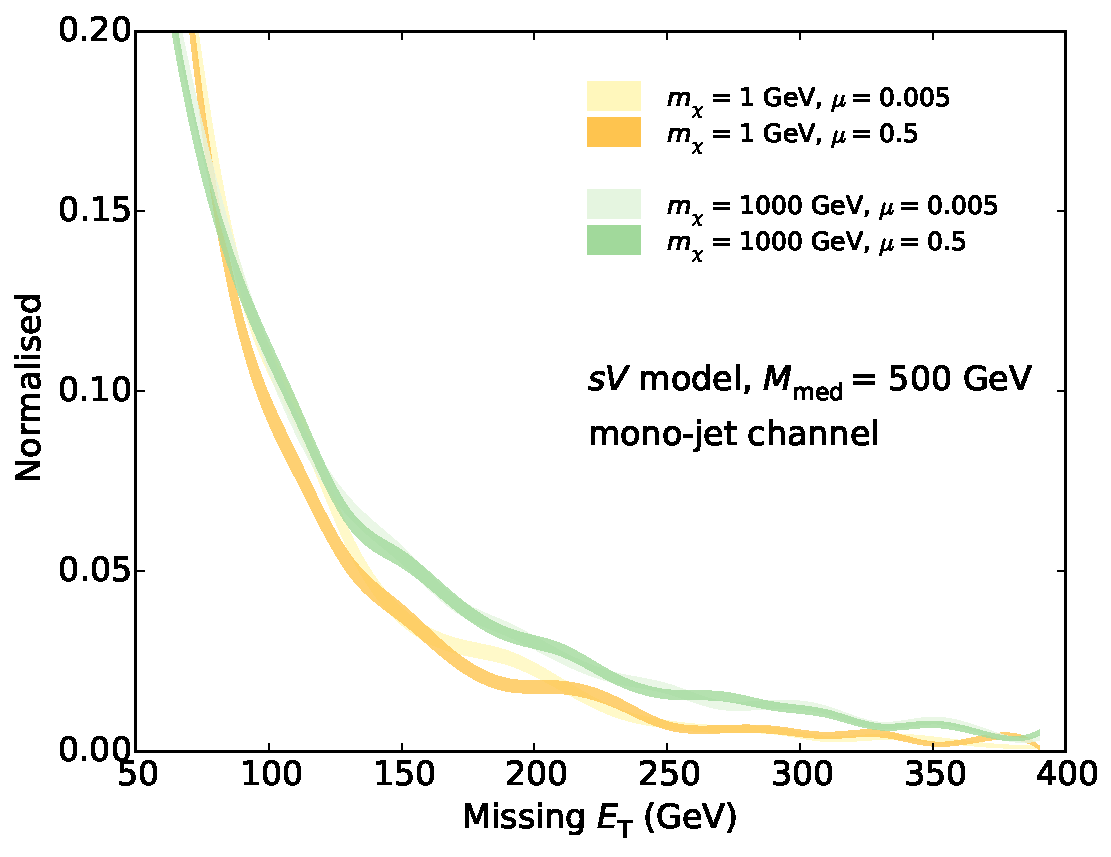
\includegraphics[width=0.495\textwidth]{figures/MET_monojet_SVD.pdf}
    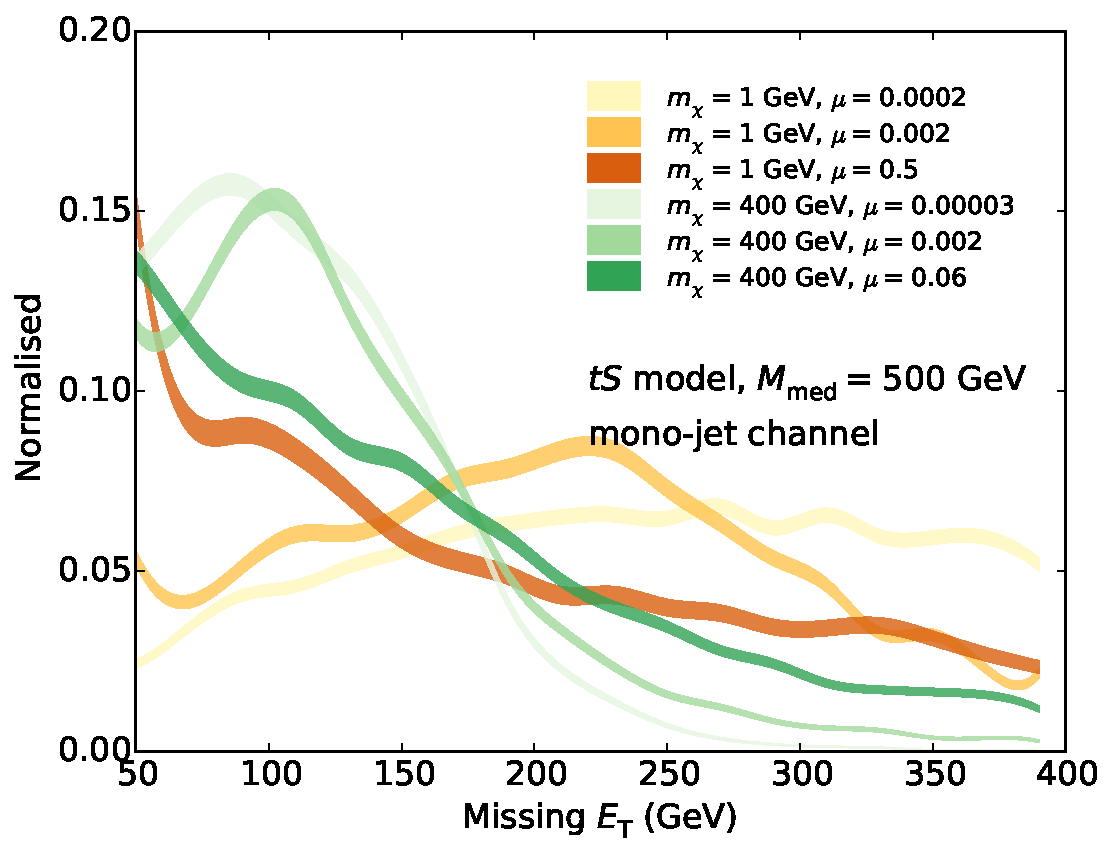
\includegraphics[width=0.495\textwidth]{figures/MET_monojet_TSD.pdf}
    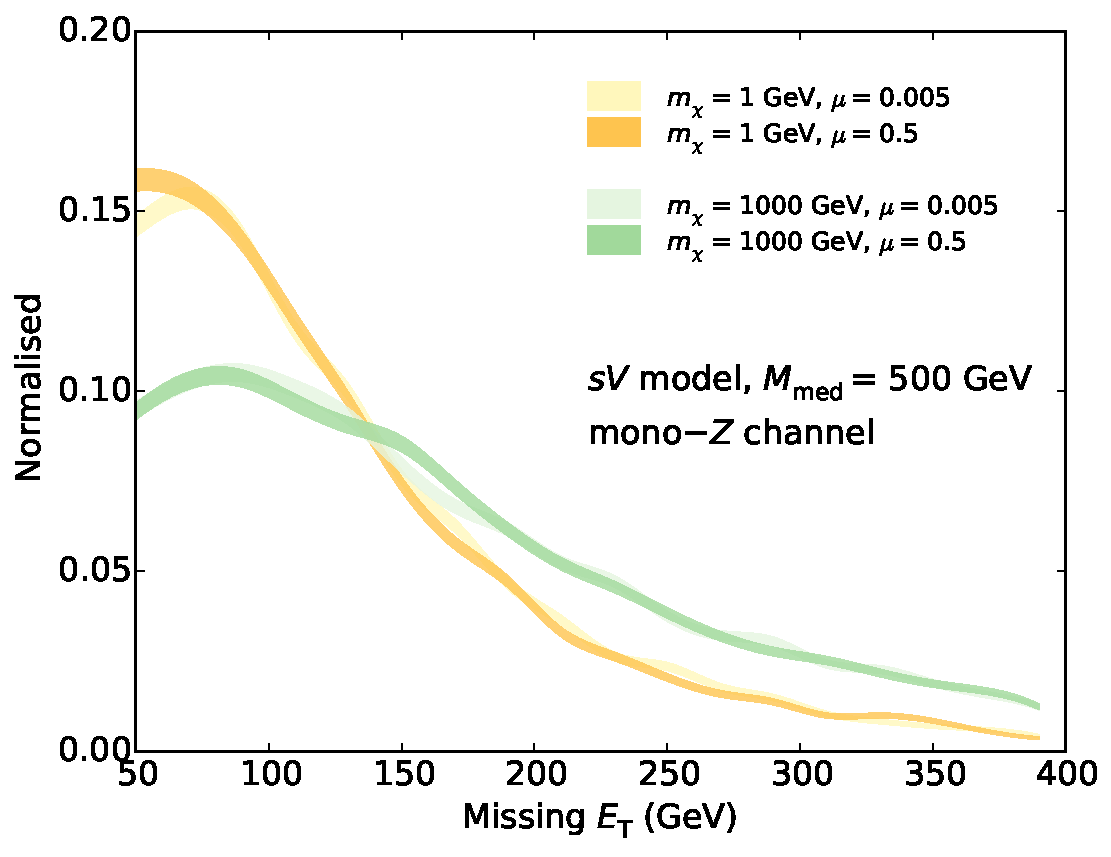
\includegraphics[width=0.495\textwidth]{figures/MET_monoZ_SVD.pdf}
    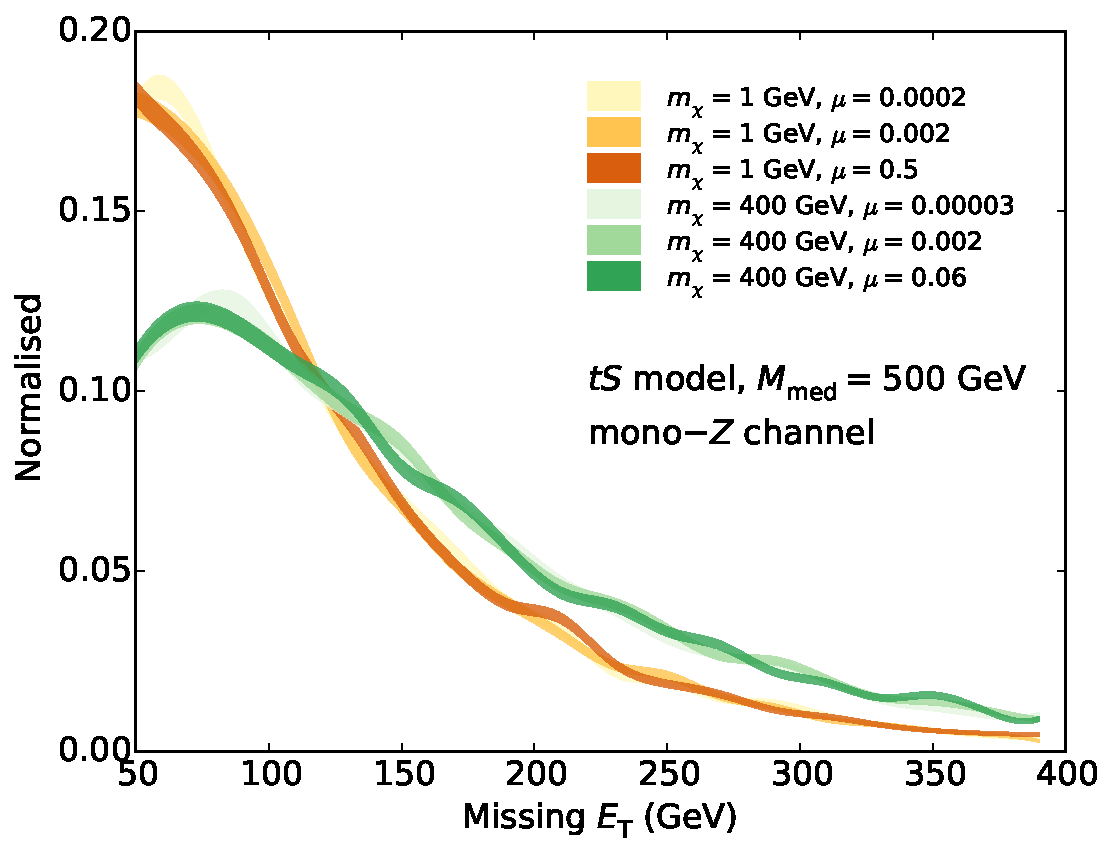
\includegraphics[width=0.495\textwidth]{figures/MET_monoZ_TSD.pdf}
    \caption{The $\met$ distribution of the $sV$ and $tS$ models in the \monojet and \monoZ channels, for some exemplary masses. The parameter $\mu$ is defined as $\Gamma / \Mmed$, and is used to demonstrate the impact of a changing width; the $tS$ model in the \monojet channel shows a clear width-dependence, while all other model/channel combinations show behaviour that is independent of the width for the phase space considered. The widths are obtained with couplings of 0.1, 1 and 5 where $\mu < 0.5$ remains true.}
    \label{fig:MET_dists}
  \end{center}
\end{figure}
